\documentclass{article}
\usepackage[top=1in, bottom=1in, left=1in, right=1in]{geometry}
\usepackage{fancyvrb}
\usepackage{multirow}
\usepackage{graphicx}
\usepackage{enumerate}
\DefineShortVerb{\|}
\pagenumbering{gobble}

\usepackage{relsize}
\usepackage{lipsum}


\def\ifmonospace{\ifdim\fontdimen3\font=0pt }
\def\C++{% 
  \ifmonospace{C++}
  \else{
	\kern-.3em C\kern-.05em\raise.4ex\hbox{\relsize{-3}{\bf ++}}\kern-.3em 
        }
  \fi
  \spacefactor1000
}

\usepackage{titlesec}
\titleformat{\section}[block] {\normalfont\bfseries\Large}{\fbox{\thesection}}{1em}{}
\titlespacing{\section}{0pt}{*6}{*1}
\titleformat{\subsection}[block] {\normalfont\bfseries\large}{\thesubsection}{1em}{}


\begin{document}

\title{SISMID Module 12\\Lab 1: EpiFire Tutorial}
\author{Thomas J. Hladish and Joel C. Miller}
\date{July 2016}
\maketitle


\section[]{What's EpiFire?\footnote{This software is described formally in T. J. Hladish, E. Melamud, L. A. Barrera, A. Galvani, and L. A. Meyers. EpiFire: An open source \C++ library and application for contact network epidemiology. \textit{BMC Bioinformatics}, 13(76), May 2012.}}

EpiFire is an open source program for simulating epidemics on contact networks.  You can either load your own network or generate a network, then choose a simulation and run it a bunch of times.  EpiFire will automatically generate plots summarizing the simulated epidemics.

EpiFire is implemented in \C++ using Qt5, and is available for Linux (as source code), Windows, and OS~X.  Installation files can be downloaded from |github.com/tjhladish/EpiFire/releases| and source code is available at |github.com/tjhladish/EpiFire/|.  

\section{The interface}

The EpiFire graphical interface is divided into two halves: the left side is the ``control panel,'' and the right is where plots are drawn that summarize any epidemics you've simulated.  Let's begin in the upper left.

\subsection{Choose a network}

Since EpiFire works by simulating an epidemic on a contact network, we need to tell it what kind of network to use.  There are two options: you can generate a network, or load one that you have on your computer.  The EpiFire graphical interface only supports undirected networks, although directed graphs are supported in the programmatic interface.

\subsubsection{Network source: Generate}

If you choose to generate a network, there are a several decisions to make.  How big should the network be (``Number of nodes'')?  And how should it be connected?

In order to connect a network, EpiFire needs to know how many neighbors each node should have.  The number of neighbors 
a node has is called its \textit{degree}. If we tally all of the degrees that all of the nodes in a network have, as in 
a histogram, we have the \textit{degree distribution}.  If you tell EpiFire what degree distribution you want a network 
to have, EpiFire will randomly sample from that distribution once for every node in the network.  Once all of the nodes
have been assigned a degree, EpiFire does its best to find a way to randomly connect them given those degrees.  

EpiFire will not allow nodes to be connected to themselves, and no pair of nodes can be connected more than once.  This 
means that \textbf{some degree distributions and sets of degrees cannot produce a valid network.}  To understand why, 
imagine that you have a network of five nodes, and one has a degree of six.  Since each node can have at most four 
neighbors, this network cannot be connected.  Similarly, a network of three nodes, where each node has a degree of one 
cannot be connected\textemdash one node will be left without a neighbor.

\pagebreak
You can choose among the following degree distributions\footnote{Poisson, exponential, and power law distributions are 
right-truncated at network size - 1 since that's the largest possible degree, or as soon as the normalized probability 
of a given degree drops below $10^{-15}$.  Continuous distributions are discretized by evaluating the PDF at integer
values and then normalizing.}: \begin{enumerate}
 \item Poisson(lambda):
			 \begin{center}
				$Pr\{degree = x\} = \frac{\lambda^x e^{-\lambda}}{x!}$
                         \end{center}
The Poisson distribution is observed in Erd\H{o}s-R\'{e}nyi random networks.  Lambda is both the mean value and the variance of this distribution; if lambda is less than 3, there will be many nodes with small degree and a few with large degree; once lambda is greater than about 10, the distribution is bell-shaped (approximately Gaussian).

\vspace{15pt}

 \item Exponential(beta):
			 \begin{center}
				$Pr\{degree = x\} = \beta e^{-\beta x}$
                         \end{center}
Exponential distributions always have more nodes with degree 1 than any other.  The distribution starts at beta on the y-axis, and asymptotically approaches zero on the x-axis. The larger beta gets, therefore, the lower the mean degree becomes.  EpiFire uses a truncated exponential distribution so that you don't end up with any disconnected (degree zero) nodes.

\vspace{15pt}

\item Power law(alpha, kappa) with exponential cutoff:
			 \begin{center}
				$Pr\{degree = x\} = x^{-\alpha} e^{-x/\kappa}$
                         \end{center}
Power law distributions generally have more nodes with degree 1 than any other.  Power law distributions have long right tails; $\kappa$ determines how quickly the tail tapers.  The mean of the resulting degree distribution will vary with $\kappa$, and inversely with $\alpha$.

\vspace{15pt}

\item Urban

The urban degree distribution\footnote{based on data from Meyers LA, Pourbohloul B, Newman MEJ, Skowronski DM, Brunham RC: Network theory and SARS: predicting outbreak diversity. \textit{J Theor Biol} 2005, 232:71–81.} is a semi-empirical distribution (with mean $\approx$ 16.7) intended to describe the spread of a respiratory pathogen in an urban population.


\vspace{15pt}
\item Constant(fixed degree)

If all nodes have the same degree (called a degenerate distribution) and are randomly connected, the resulting network is said to be a \textit{random regular network}.  Note that the algorithm used by EpiFire to produce random regular networks is only efficient if the desired degree is small relative to the number of nodes.  If you want to create a complete graph, where all nodes are connected to all others, this is best done by choosing the Poisson distribution and setting lambda equal to \textit{network size} - 1.

\vspace{15pt}
\item Small world

Watts and Strogatz (1998)\footnote{Watts DJ, Strogatz SH: Collective dynamics of “small-world” networks. \textit{Nature} 1998, 393:440–442.} described a class of networks that have \textit{high clustering} and \textit{low average shortest path length}.  In non-technical terms, high clustering means that the network has a lot of triangles; in real life, this is like saying that your friends generally know each other.  If a network has a low average shortest path length, this means that individuals tend to be connected by surprisingly few intermediaries.

Watts-Strogatz small-world networks are parameterized with the mean degree $k$ and the fraction of edges to be shuffled $p$.  Initially, all nodes are connected to form a ring, where every node is connected to its $k$ nearest neighbors.  With probability $p$, each edge is randomized.

\end{enumerate}
\subsubsection{Network source: Load from file}

Networks can be imported into EpiFire as comma-, space-, or tab-delimited files.  The default is to use the comma-delimited or ``comma separated value'' (CSV) format.  Each line in the file represents either a node or a pair of nodes, connected by an edge.  Consider the following edge list:

\begin{Verbatim}
A,B
C,B
C,A
D
\end{Verbatim}

When imported, this would connect nodes A, B, and C in a triangle, and node D would be added to the network but would have no edges.  Order is not important, since EpiFire currently supports only undirected networks.  Note that node names are taken to be unique, so a node will only be created the first time its name appears in the file, but edges are not unique; including |A,B| \textit{and} |B,A| in the file would result in the nodes being connected by two edges.

Node names may contain any characters except commas and end-of-line characters.  Extra whitespace (spaces, tabs, readlines, and newlines) before and after node names are stripped and ignored.

If EpiFire has a network loaded that is from a file, the ``Number of nodes'' line will display the size of the network, and the source filename will be shown; if the network is deleted or replaced with a generated network, these values are reset.

\subsection{Design a simulation}

Once a network is either generated or loaded from a file, you can simulate an epidemic on that network.  All simulations work in the same fundamental way: Initially everyone in the network is susceptible.  One or more individuals are randomly selected to become infectious; pathogens spread probabilistically from these individuals along the network structure, infecting and spreading from others in turn.  Infectious individuals eventually recover and resist being reinfected. The epidemic ends when the last infectious person recovers.  Currently EpiFire only supports the $susceptible \rightarrow infectious \rightarrow recovered$ progression of states.

\subsubsection{Simulation types}
EpiFire supports two types of epidemic simulations: percolation and chain binomial.  Both types, if parameterized properly, will predict exactly the same distribution of final epidemic sizes.  Percolation simulations are somewhat faster and accurately predict who will get infected, but not when exactly an individual is likely to get infected, or which neighbor that transmission came from.  Percolation epidemic curves have simulation steps, sometimes called \textit{epidemic generations}, as ``time'' units, which may be hard to interpret as conventional time units.

Chain binomial simulations, on the other hand, are more computationally intensive but can accurately predict chains of transmission (who infected whom).  Chain binomial epidemic curves have time units that correspond to the units of the \textit{infectious period} parameter; in other words, if the infectious period is 5 days, then the epidemic curve time unit is ``days.''

\pagebreak
Here is a table summarizing the differences between percolation and chain binomial simulations:

\UndefineShortVerb{\|}
\begin{figure}[h]
\begin{center}
% use packages: array
\begin{tabular}{|l|l|l|}
\hline
& Percolation & Chain binomial \\ \hline
Parameters & transmissibility $T_{P}$ & infectious period $d$, transmissibility $T_{CB}$\\
Predicts final epidemic size & yes & yes\\ 
Predicts epidemic probability & yes & yes\\ 
Predicts epidemic curve & approximately & with resolution of infectious period units\\
Predicts chain of transmission & no & yes\\
Number of times edges are tested & 1 & equal to infectious period $d$\\ 
Transmissibility & $T_{P} = 1 - (1-T_{CB})^d$ & per time-step probability $T_{CB}$\\ 
Running time & faster & up to $d$ times slower\\ 
Time step units & simulation steps & infectious period units \\
\hline
\end{tabular}
\caption{Comparison of percolation and chain binomial simulations}
\end{center}
\end{figure}
\DefineShortVerb{\|}

\subsubsection{Infectious period (chain binomial only) and transmissibility}
The infectious period parameter is the length of time that individuals will remain infectious.  It is numerically equal to the maximum number of times an edge between an infectious and susceptible pair of individuals is tested for transmission.  If a given pathogen has an infectious period of 1 week, that can be expressed as 1 (week), 7 (days), 168 (hours), etc.; the transmissibility (per time\textendash step probability of transmission) must be adjusted accordingly, and whatever units you use are the units of the epidemic curve horizontal axis.  The conversion is as follows:

\vspace{15 pt}

$T_{CB, f} = 1 - (1-T_{CB, d})^{d/f}$

\vspace{15 pt}

where $T_{CB, f}$ is the transmissibility for an infectious period divided into $f$ time steps, and $T_{CB, d}$ is the original transmissibility when using $d$ time steps.  When $f$ is 1, this calculation yields the percolation transmissibility.

\subsubsection{Expected R-zero}
R-zero, called the basic reproductive rate, is the expected number of secondary infections caused by each infection early in an epidemic.  If R-zero is less than 1, we would predict that an epidemic cannot occur.  As R-zero increases, epidemics tend to become larger and more probable, although they can still stochastically fail to occur, or even deterministically fail to occur if the initial infection is introduced outside of the giant network component, e.g. in a disconnected node.

EpiFire provides the expected R-zero calculation\footnote{calculated as in Meyers LA: Contact network epidemiology: Bond percolation applied to infectious disease prediction and control. \textit{Bull Am Math Soc} 2007, 44:63–86.} based on the degree distribution of the network in memory, and $T_{P}$ or $T_{CB, 1}$ (these are equivalent).  It provides one basis for comparing different sets of parameters.

\subsubsection{Initially infected}
This is the number of infectious individuals that will begin the epidemic.  Nodes are selected randomly without replacement.  Generally, as this number increases, the probability of an epidemic also increases, given that the expected R-zero is greater than 1.

\subsubsection{Number of runs}
Although you are welcome to click ``Run Simulation'' every time you want to run a simulation, sometimes you might want a little more automation.  When you click ``Run Simulation,'' this parameter determines how many repetitions will be performed.

\subsubsection{Retain data between runs}
If you do not wish to accumulate data as you run the simulator, uncheck this box.

\subsection{Log window}
The large text box on the lower left side is where all important messages will end up about the status of EpiFire.


\subsection{Profit!}
Now that you have selected a network and a simulation, this is where the buttons are located that allow you to control what happens next. The ``Generate Network'' and ``Import Edge List'' buttons are only displayed when ``Generate'' and ``Load from file,'' respectively, have been selected in the ``Network source'' drop-down menu.

\UndefineShortVerb{\|}
\begin{figure}[h]
\begin{center}
% use packages: array
\begin{tabular}{|l|l|}
\hline
Button & Function \\ \hline
Clear Network & Delete the network in memory\\ 
Clear Data & Delete all generated data\\ 
Analyze network & See section 2.6\\ 
Draw network & Render the network as image ( $< 10^4$ nodes; $< 10^3$ recommended)\\
Generate network & Generate a new network, replacing any previous network\\ 
Import Edge List & Open file dialog to import a network from a CSV file\\ 
Run Simulation & Conduct the specified simulation on the network in memory\\ 
\hline
\end{tabular}
\caption{Control panel buttons}
\end{center}
\end{figure}
\DefineShortVerb{\|}


\subsection{The data plots}
On the right side of the application window are three boxes; this is where the data plots are drawn if you have run simulations.  The plots can be resized by resizing the application window, and by clicking and dragging the horizontal dividers between the plots.

\textbf{All plots can be exported as PNG files by double-clicking on the plot.  Data used to generate the plots can be exported as CSV files by right-clicking the plots.}

All example plots below were created using a Poisson(5) network of 10,000 nodes, and a chain binomial simulation with infectious period = 5, transmissibility = 0.06, number initially infected = 3, and 100 runs.
\pagebreak
\subsubsection{Node state plot (top)}
\begin{figure}[h]
\begin{center}
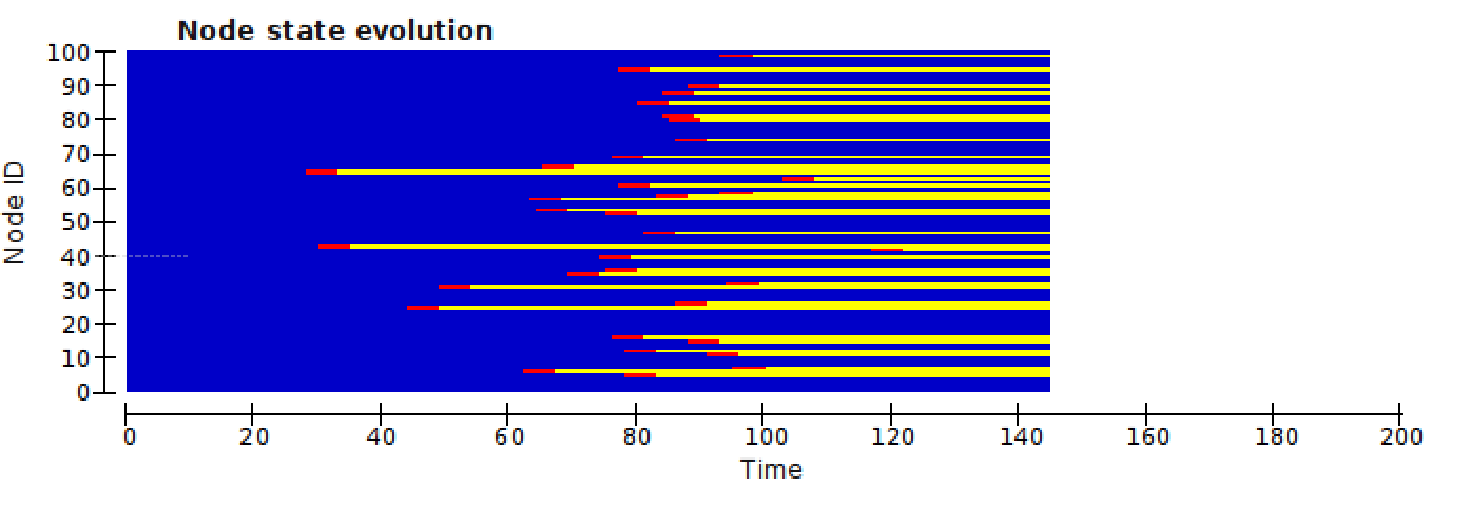
\includegraphics[width = 6in]{states_example.pdf}
\caption{A node state plot}
\end{center}
\end{figure}
This plot displays the progression of disease states from the most recent simulation run for 100 arbitrarily selected nodes in the network. Each node is represented by one row; time progresses from left to right.  Blue represents susceptible; red, infectious; and yellow, recovered. The scale of the horizontal axis is the same as the range of the most recently generated epidemic curve.  In other words, this plot shows what a sample of nodes experienced during the epidemic shown in red in the epidemic curve (middle) plot.  If your network has fewer than 100 nodes, the bottom portion of this plot will be solid blue.

\subsubsection{Epidemic curve plot (middle)}
\begin{figure}[h]
\begin{center}
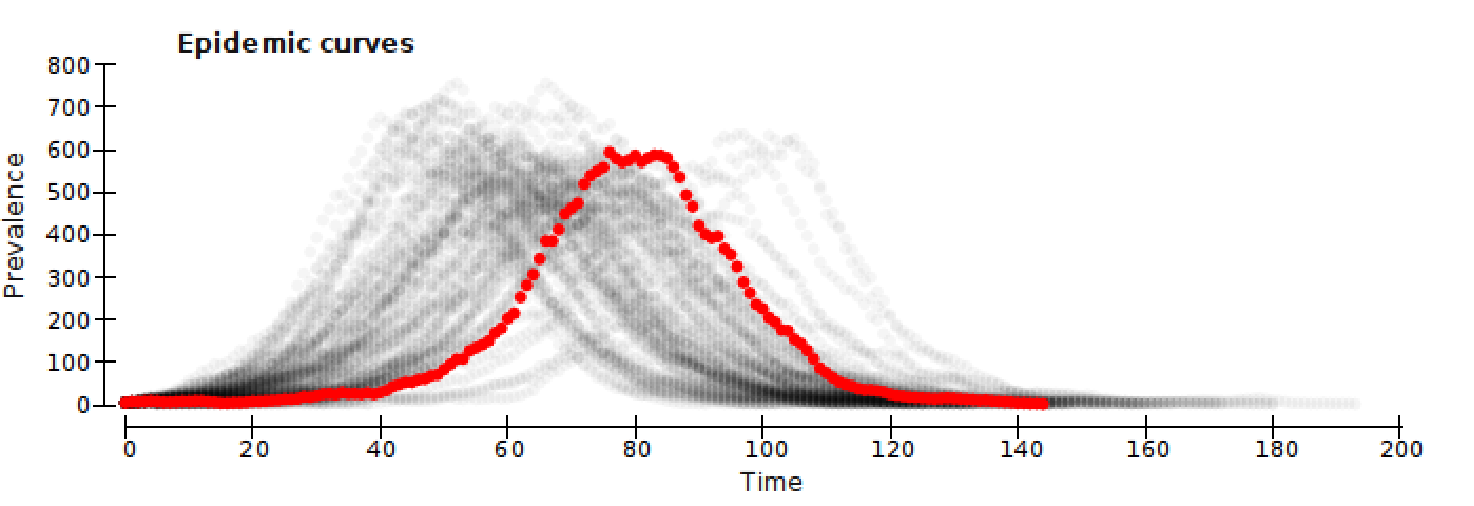
\includegraphics[width = 6in]{curves_example.pdf}
\caption{An epidemic curves plot}
\end{center}
\end{figure}
This is usually the most interesting view of the simulation results.  An ``epidemic curve'' is a time series describing how many nodes were in the infectious state at each point in time.  The vertical axis is an absolute count of individuals, and the horizontal axis is in time steps; for chain binomial simulations, the units are the same as for the infectious period, while for percolation simulations the units are simulator steps.

The most recent simulator run is plotted in solid red.  Past runs are displayed in semi-transparent gray; as more data accumulates, the gray becomes more transparent.  In this way, past runs effectively produce a density plot, showing you both the range of possible epidemic curves, while the most probable trajectories are the darkest.

Note: since chain binomial and percolation simulations produce epidemic curves that cannot be compared, the epidemic curve plot is cleared when you change simulation types.

\subsubsection{Epidemic size histogram (bottom)}
\begin{figure}[h]
\begin{center}
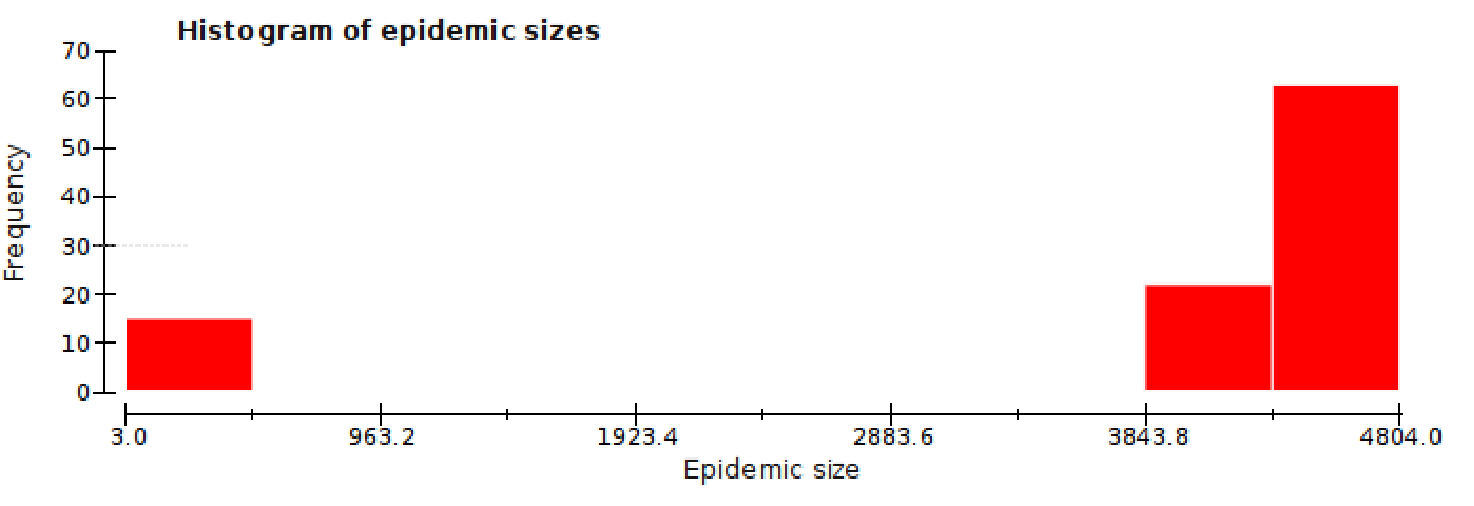
\includegraphics[width = 6in]{hist_example.pdf}
\caption{Histogram of final epidemic sizes}
\end{center}
\end{figure}
The histogram of epidemic sizes displays the distribution of final epidemic sizes.  The horizontal axis is divided into bins representing ranges of epidemic sizes; the vertical axis is the number of observed epidemics within each bin.  This plot doesn't become interesting until you have performed several simulation runs, since the data cannot be divided into more bins than the number of data points.

The epidemic size histogram can be particularly useful in estimating the frequency of successful versus failed epidemics.  If the histogram is strongly bimodal after performing many repetitions, this is a likely explanation.

\subsection{Network analysis}
Since network structure plays such an important role in determining what happens when a pathogen is introduced to a population, it is useful to be able to calculate some basic network statistics.  By clicking the ``Analyze Network'' button, you can open the network analysis dialog.

\subsubsection{Network statistics}
While it is beyond the scope of this tutorial to explain how each statistic is calculated, here is an interpretation:

\UndefineShortVerb{\|}
\begin{figure}[h]
\begin{center}
% use packages: array
\begin{tabular}{|l|l|}
\hline
Statistic & Interpretation \\ \hline
Node count & number of nodes in the network\\ 
Edge count & number of edges in the network\\ 
Mean degree & average number of neighbors each node has\\ 
Largest component & number of nodes in the largest interconnected region of the network\\ 
Component count & number of disconnected regions of the network\\ 
Transitivity & clustering coefficient; one measure how independent node connections are\\ 
Diameter & length of the shortest path between the most distant pair of nodes\\
Mean shortest path & average shortest path among all pairs of nodes\\
\hline
\end{tabular}
\caption{Control panel buttons}
\end{center}
\end{figure}
\DefineShortVerb{\|}

Since path length is undefined for nodes that are in separate components, the diameter and mean shortest path statistics are calculated using only the nodes in the largest component.

\subsubsection{Degree distribution plot}
\begin{figure}[h]
\begin{center}
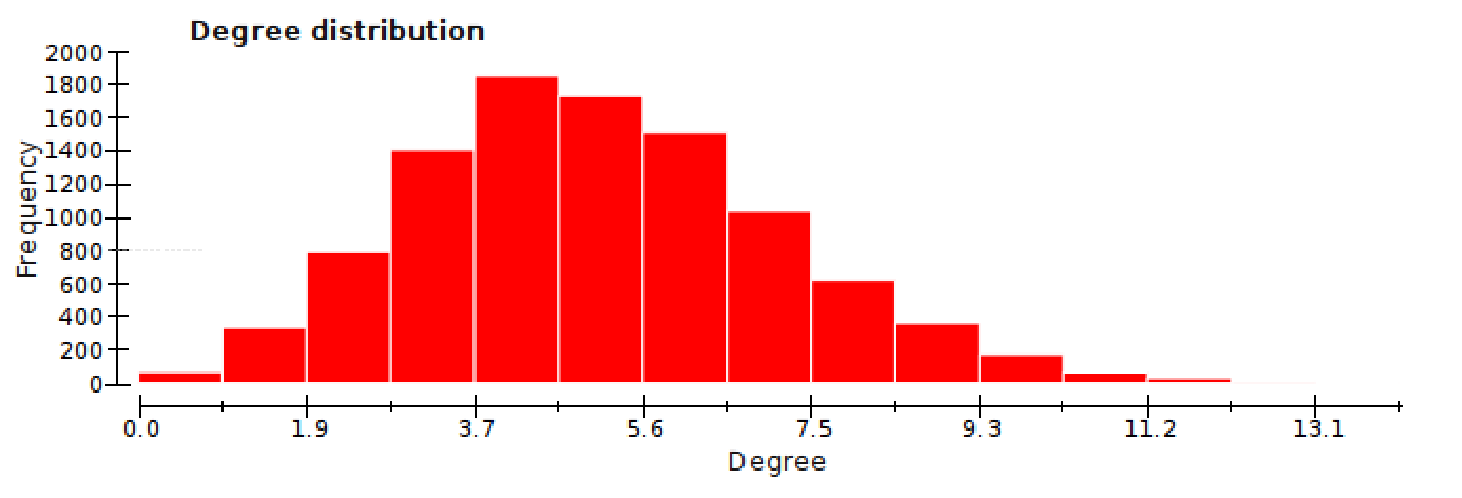
\includegraphics[width = 6in]{deg_example.pdf}
\caption{Degree distribution for a Poisson(5) network with 10,000 nodes}
\end{center}
\end{figure}
A node's degree is the number of edges it has; by counting the number of nodes having each possible degree, we can determine the degree distribution.  In this histogram, the horizontal axis is the degree, and the vertical axis is the number of nodes having that degree.  As with the other plots, this plot can be saved as a PNG by double-clicking, and the data used to generate the plot can be saved by right-clicking.


\section{EpiFire exercises}

\subsection{Explore}
Before we start doing real exercises, take a look around.  Click ``Generate Network,'' then click ``Run Simulation'' a few times.  Try changing some parameters, and see what effect they have.  Remember, if you want to clear the plots, click ``Clear data,'' and if you want to do a bunch of simulations quickly, try changing the simulation type to ``Percolation,'' and change the number of runs to a bigger number.

You can also use "Draw network" to visualize some smaller networks (probably $<10^3$ nodes, depending on your computer) and simulations.  Mouse scrolling or +/- will zoom in/out, holding ENTER or RETURN causes the layout optimization algorithm to continue running, and you can drag around with your mouse.  You can drag multiple nodes by drawing a box around them first with your mouse.

\subsection{Poisson vs power law}
Let's investigate the effects of having a more homogeneous degree distribution (Poisson), versus a more heterogeneous one (power law).  For this exercise, switch the simulation type to ``percolation,'' since we will only be looking at final epidemic size; this will speed things up.

Generate a 10,000 node power law network with alpha = 1.5 and kappa = 100.  
\begin{itemize}
 \item What is the expected R-zero?

 \item Does this mean that epidemics are possible?

 \item Run this 100 times, by editing the ``Number of runs'' box.  What fraction of the time does an epidemic result?  This is the number of runs in the right-hand mode of the histogram, divided by the number of runs you did.

 \item When epidemics do occur, how big do they tend to be?
\end{itemize}

Let's find a Poisson-distributed network that has the same (or very similar) R-zero, \textbf{keeping transmissibility the same}.  To do this, make note of the value of R-zero for your power law network, and then try adjusting the value of lambda higher or lower, in order to get at least the first two digits of R-zero to match.  In order to generate a new network and recalculate R-zero, click ``Generate Network.''\footnote{Hint: The correct lambda should have a value between 50 and 60.}

\begin{itemize}
 \item Clear the plots by clicking ``Clear data.''  Now do 100 more runs with the Poisson network.  What fraction of the time does an epidemic result?

 \item When epidemics occur in the Poisson network, how big are they?

 \item In this exercise, we have kept the expected R-zero the same; this means that the critical transmissibility for the two networks is the same.  What does R-zero tell you?  What \textit{doesn't} it tell you?  When parameterized to have the same critical transmissibility, are epidemics bigger on a homogeneous or a heterogeneous network?

 \item Which is a better approximation of a classical mass-action model, and why?  By modifying the degree distribution and network size, we can still do better than these networks if we are trying to approximate, for example, a classical S-I-R model.  What should those changes be?
\end{itemize}

\subsection{Is the urban network a good model for influenza?}
Meyers \textit{et al.} (2005) created the urban network model with SARS in mind, but other respiratory diseases like influenza likely have similar modes of transmission.  Since the same contacts between people are important, it is reasonable to think that the underlying network structure will be similar. Let's see whether that seems to be the case.

Select ``Urban'' from the degree distribution menu, and generate a network of 10,000 nodes.  Select ``percolation'' as the simulation type, and change the transmissibility value until the expected R-zero is approximately 1.1.  This is an appropriate value of $R_e$ (the effective reproduction number) for seasonal (non-pandemic) influenza.\footnote{Strictly speaking, $R_0$ is the reproduction number for fully susceptible populations, but seasonal influenza does not circulate on fully susceptible populations because many people have some immunity from natural infection and from vaccination.  The reproduction number we observe, $R_e$, is from an epidemic spreading on a more complicated network than what are modeling here, one where transmissibilities depend on immune state.}

Now, how will we determine if this is a good network to use for influenza?  As you saw in the last exercise, using a particular R-zero value is no guarantee that epidemics will occur with a certain probability, or be of a certain size.  In a typical year 5-15\% of the United States becomes infected each year with influenza.  Remember, that is averaging urban and rural areas, and populations that did not experience an epidemic with those that did, so the average for a city is likely to be somewhat higher.
\begin{itemize}
 \item Do 1000 simulation runs with the transmissibility value you chose.  How big are the epidemics that occur?

 \item How frequently do epidemics occur?
\end{itemize}

The frequency of these epidemics is a problem: real urban populations experience influenza epidemics in most years.  One solution is to introduce more infections in the beginning by changing ``initially infected''\textemdash this is the number of randomly selected individuals that spark the epidemic.  Change the number initially infected so that epidemics occur at least 80\% of the time.

Think about why changing the initial number of infected individuals has this effect.  What is the effect when the network is a single component?  What about when the network has many components, perhaps one giant component and many small ones?

Finally, try a similar process with other degree distributions.  Are there others that can reproduce reasonable epidemics, given an R-zero value of 1.1?


\subsection{Identifying epidemics}
We all have some notion of what we mean by the word \textit{epidemic}, but a precise definition that applies across all areas of epidemiology is not possible.  In stochastic network models, epidemics might fail to occur when they are likely, and if a highly-connected individual is infected early on, a large number of people might become infected even if the expected R-zero is less than 1.

Practically speaking, if 8 people become infected in a population of 10,000, we would not call that an epidemic.  If 80\% of those 10,000 people become infected, that is definitely an epidemic.  What if it is 8 people, or 80\% of a population of just 10?  The way we think about epidemics is somehow connected to population size.

\begin{itemize}
  \item Generate a 100-node network using the urban degree distribution, and select a percolation simulation with transmissibility = 0.07.  Run 1,000 (or more) simulations.  What fraction of simulations would you say resulted in an epidemic? Click "Simulation results analysis" in the Results menu to open the results analysis dialog.  Make note of the mean number infected in all simulations.  If you would say that some epidemics occurred, adjust the outbreak/epidemic threshold accordingly, and make note of mean number infected in outbreaks and in epidemics, respectively.
  
  \item Click "Clear data" in the main application window to remove these results, and repeat the exercise for a 1,000-node network, keeping all other settings the same.  What fraction of simulations resulted in an epidemic?  You should have observed some epidemics: adjust the outbreak/epidemic threshold if necessary, and make note of mean number infected in outbreaks and in epidemics.  Calculate the mean fraction infected in epidemics and write it down.

  \item Click "Clear data" in the main application window to remove these results, and repeat the exercise one more time for a 10,000-node network.  What was the mean number infected in outbreaks, and the mean fraction infected in epidemics?
  
  \item What generalizations can you make about how changing population size affects:
  \begin{itemize}
    \item The number of people and fraction of population infected in an outbreak (non-epidemic)?
    \item The number of people and fraction of population infected in an epidemic?
  \end{itemize}
  
  \item Let's look at one more scenario: clear the data, and generate a new 1,000-node network, but this time change the transmissibility to 0.05 and the number initially infected to 50.  What is the expected R-zero?  Should epidemics be possible?  Run 1,000 simulations.  How does the mean number and fraction infected compare to the runs with the 1,000-node network and a higher transmissibility?  Having multiple introductions, each producing an "outbreak" can make it difficult to say what we would call an epidemic.  A theorist might say no epidemics occurred, while a public health official might say epidemics always occurred.  If you repeat this exercise with a large population, however, you should find that the number infected does not increase proportionally.
\end{itemize}

Using analytical methods from network epidemiology, we can sometimes calculate the expected final size for an infinite population, and that may provide some guidance when choosing what to call an epidemic in a stochastic setting.  If it is unclear from examining results what should be called an epidemic, it may help to vary the population size to see how dynamics changed.


\subsection{What drives stochasticity?}
Stochasticity is an important topic in epidemiology, in large part because of our desire to plan ahead and respond appropriately for potential epidemics.  Sometimes, the problem is a lack of good information\textemdash you can't predict something you don't know about\textemdash and other times, even with good information, prediction is very difficult, and therefore appropriate intervention is as well.  To illustrate the difference, consider that I cannot predict where the planets will be in the night sky one month from now (I personally lack the information), even though their movement can be easily predicted; on the other hand, weather forecasters struggle to predict next month's forecast even with huge amount of information regarding current weather patterns and past trends.

Let's examine some stochastic phenomena in EpiFire.
\begin{itemize}
 \item Click ``Default settings'' and ``Clear data.''  Generate the default network, a Poisson(5) network with 10,000 nodes.
 \item Click ``Run simulation'' several times.
\end{itemize}

Notice that epidemics, when they occur, have a smooth bell shape.  The epidemic curve looks like it could have been generated using a differential equation model. The epidemics don't, however, always occur at the same time. Change the number ``Initially infected'' to 20, and run several more simulations.  
\begin{itemize}

 \item What happened?  
 \item Are epidemics bigger?  
 \item Is the timing different?  
 \item Are they more predictable or less predictable?
\end{itemize}
Change the Poisson parameter lambda to 4.  This reduces the average number of neighbors each nodes has by 1.  Generate a new network, and run several simulations.  Are there major differences?

Now change the Poisson parameter to 3.  Generate a new network, and run several simulations.  What change do you observe now?  If you haven't done so already, try clearing all of the previous data (to clear the plots), and run several more simulations.

Continue to investigate how parameters affect stochasticity and the predictability of epidemics.  What changes have a big impact?

\subsection{Exploring a novel network}
One exciting aspect of network modelling is studying the properties of novel empirical networks.  Sometimes the intuition
we develop from studying idealized, mathematically-friendly networks is confirmed, and other times we are pushed to develop
new methods and metrics.  This exercise is intended to be open-ended and a little bit challenging.

Download |mystery_net.csv| and import the edge list into EpiFire.  This mystery network is based on actual interactions
between people. Later you will learn the source and how it was constructed, but for now, please investigate the network
without preconceptions.

First, answer some basic questions:
\begin{itemize}
 \item How big is the network?
 \item What is the mean degree?
 \item What is the minimum and maximum degree? [NB: One simple, if inelegant, way to determine this is to look at the
 range of the degree distribution plot in the network analysis dialog.]
 \item How would you characterize the degree distribution?
 \item How many components are there?
 \item This is a big enough network that it's not worth trying to calculate the diameter and mean shortest path of the
 largest component.
\end{itemize}

Hypothesize a little:
\begin{itemize}
 \item What kinds of mundane interactions would or would not plausibly fit the information you have so far?
 \item What plausible explanations are there for the existence of multiple components?
\end{itemize}

Simulate some epidemics: Try a chain binomial simulation with infectious period = 5, transmissibility = 0.05, initally infected = 5, and number of runs = 1.  Click ``Run Simulation'' until you have seen at least 10 epidemics.
\begin{itemize}
 \item Are these curves smooth, or noisy/stochastic?  Does that match your expectations given the expected R-zero value?
 \item Did you observe any surprising features in the epidemic curves? (If not, talk to me!) 
 \item How do the observed epidemics compare with the predicted epidemic sizes under the mass action and network models?
 \item What kind of network properties could lead to epidemic sizes and dynamics and like those you observed?
 \item How would you test your hypotheses?
 \item Explore other parameter values and see how the dynamics change.
\end{itemize}

\end{document}
